\documentclass[11pt, oneside]{book}
\newcommand{\version}{v1.02}

\usepackage[pdftex,a4paper]{geometry}
\usepackage{pdfpages}
\usepackage{graphicx}
\usepackage{amssymb}
\usepackage{gensymb}
\usepackage{eurosym}
\usepackage{ifthen}
\usepackage{float}
\usepackage{calc}
\usepackage[export]{adjustbox}% http://ctan.org/pkg/adjustbox
\usepackage{xstring}
\usepackage{multicol}
\usepackage[framemethod=TikZ]{mdframed}
\usepackage[T1]{fontenc}

% Switch font comprehensively
\usepackage[scaled]{helvet}
\renewcommand\familydefault{\sfdefault} 

% Use as much of the page as we can.
\pagestyle{empty}
\setlength{\parindent}{4em}
\setlength{\parskip}{1.2em}
\setlength{\textheight}{28cm}
\setlength{\textwidth}{19cm}
\setlength{\hoffset}{-2cm}
\setlength{\voffset}{-2cm}

% DECAL function
%
% The decal function takes 5 inputs and extracts a symbol from the Italian ISO document that is included in this repository. The function then displays the symbol together with the title and warning text.
%
% Parameters:		#1 Page with the symbol on it in the document.
%			#2 Title
%			#3 Y height on the page.
%			#4 X location on the page. (not sure on this)
%			#5 Warning subtext
%
\newcommand{\decal}[5]{
\begin{minipage}{\linewidth}
	\begin{minipage}[t]{0.3\textwidth}
	       \vspace{0pt}
	       % The ISO document has a 'gutter' - so we shift the X a bit on the left/right page.
	       %
		\ifthenelse{\isodd{#1}}{ %if the pagenumber is odd, use this location for the image
			\includegraphics[width=0.9\textwidth,page=#1,viewport=103 #3 291 #4,clip=true]{13GR_PistopioimeniSimansi_ISO_7010.pdf}
		}{ %else (because the pagenumber is even), use this location for the image.
			\includegraphics[width=0.9\textwidth,page=#1,viewport=70 #3 261 #4,clip=true]{13GR_PistopioimeniSimansi_ISO_7010.pdf}
		}
	\end{minipage}
	\begin{minipage}[t]{0.6\textwidth}
		\setlength{\parindent}{4em}
		\setlength{\parskip}{1.2em}
	       \vspace{0pt}\raggedright
		{\LARGE \textbf{#2}} %include title text in bold and such
	
		#5 %include warning subtext
		\vspace{0.5cm}
	\end{minipage}
\end{minipage}
}


% Some home made symbols which are not part of the official ISO list of symbols:
%
% Two person symbol
\newcommand{\twopersons}{
\raisebox{-.5\height}{\includegraphics[width=6mm]{File:Aiga_toiletsq_men}}\textbf{x 2} 
}

% Some home made symbols which are not part of the official ISO list of symbols:
% Clock with 7-19 symbol
%
\newcommand{\seventoseven}{
\raisebox{-.5\height}{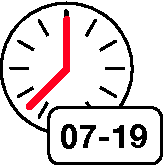
\includegraphics[width=10mm]{clock-limits}}
}


% Define classes for Action, Prohibit and Warn. These each take three inputs.
%
% Turns out that the symbols extracted from the ISO document with \decal are a bit 
% shifted in the Y position or size depending on what class they are. So we split
% them into the three sections that have height differences.
%
% Parameters:		Page with the symbol on it. Actual pagenumber, not the number on the page!
%			Title
%			Warning subtext
%
\newcommand{\action}[3]{\decal{#1}{#2}{520}{715}{#3}}
\newcommand{\prohib}[3]{\decal{#1}{#2}{495}{690}{#3}}
\newcommand{\warn}[3]{\decal{#1}{#2}{520}{715}{#3}}

%% Command to create a round box to call extra attention to something.
%%
\newcommand{\smallicontext}[2]{%
\begin{mdframed}[roundcorner=4pt] 
\begin{tabular}{lp{0.8\linewidth}}
#1 & #2 \\
\end{tabular}
\end{mdframed}
}

% machinePage
% A full page with a machine on it. Takes 5 inputs.
%
% Params:		#1 Machine name
%			#2 Tokens for standard instrutions: Zero or more from
%				Approval	Trustee approval needed.
%				Noise		Not after 19:00
%				Two		Two people required
%				Log		use must be logged
%				Dewalt		Attach dewalt dutch extractor.
%			#3 Specific instructions - added to the above text.
%			#4 Warnings, Symbols - main symbols on page.
%			#5 Extra footer/bottom of the page text
%
\newcommand{\machinePage}[5]{%
\begin{center}
	\vspace{0cm}
	{\fontsize{50}{60} \textbf{#1}}%Machine name
 
	\action{49}{% Determines if you require approval / mandatory instructions / safety instructions
		\textbf{%
 		\IfSubStr{#2}{Approval}%
			{Instructions \& Approval Mandatory}
			{\IfSubStr{#2}{NoMandatory}{Mandatory Safety Rules}{Instruction Mandatory}}%
		}}
		{%
		\IfSubStr{#2}{NoMandatory}{}{Instruction \textbf{prior} to use is \textbf{mandatory}. Check the wiki for who can help you.}
		\IfSubStr{#2}{Approval}{You must also have a `\textbf{dangerous equipment waiver}' filed with the foundations trustees and been given \textbf{approval or card access} to use the machine.}{}
			
		#3 % added to above instructions
		
		\IfSubStr{#2}{Noise}{\smallicontext{\seventoseven}{
			Machine can only be used between 07:00 - 19:00 (be kind to our neighbours)
			}
		}{}

		\IfSubStr{#2}{Two}{\smallicontext{\twopersons}{A second person must be present during operation, have agreed to be your second, knows how to stop the machine and what to do in an emergency, including opening the door for paramedics if needed.	}
		}{}

		\IfSubStr{#2}{Log}{Report any use in the log - and \textbf{pay for it}!}{}

		\IfSubStr{#2}{Dewalt}{Be sure to attach and power on the dust extractor.}{}
	}
	\begin{multicols}{2}#4\end{multicols}
	
	\vspace{0.2cm}
	#5
%footer text at the bottom of the page.
	If a machine is not clean or appears broken - then report this to the mailing list. Clean/fix prior to use.

	\textbf{Report any damage, issues or accident within 24 hours to the mailing list.}
\end{center}
\vfill
\begin{flushright}
{\tiny \version -- \today}
\end{flushright}
\pagebreak
}







\begin{document}

%%%%%%%%%%%%%%%%%%%%%%%%%%%%%%%%%%%%%%%%%
%: Intro sheet to the hackspace
\machinePage{Bristol Hackspace}{NoMandatory}{
Observe all safety instructions. Induction or Instructions are required for some of the machines. Ask someone for help, consult the wiki or message the forum when in doubt.

Ask for instructions if you are unfamiliar on how to use a tool. This is to protect you and to protect the tool. This is a shared space -- consider others around you before using a machine; and be aware of others working nearby.  \textbf{Leave the space cleaner than you found it.}

Make sure you know where the \textbf{emergency stops and fire extinguishers} are. In case of "call 999"-type emergencies, make sure there is someone at the door to let paramedics in. If you have to stay with the wounded, jam the doors open. Bring your key(card)s with you if you have to let emergency personnel in.
}{
\action{58}{Wear protective clothing}{Wear tight fitting clothing, keep long hair tied up, no jewellery or anything else that can be caught by a machine. Consider that others may be working at the space -- and you may be in close range of their machines too.

%Be careful with gloves -- they can be caught in the machine and when made of a sturdy material, help rip your finger off. Observe the `no gloves' signs.
}
\action{56}{Wear appropriate footwear}{No sandals or similar in the wood or metal shop.}
\action{64}{Wear a mask when needed}{Especially when cutting materials such as MDF}
\action{52}{Eye protection recommended}{Also consider that hard-metal cutters and ceramics can suddenly shatter.}
\action{57}{Protective gloves recommended}{But also: be careful with gloves -- they can be caught in the machine and when made of a sturdy material, help rip your finger off. }
\action{51}{Ear protection recommended}{}
}{If something breaks or is amiss -- it is \textbf{your} responsibility to report it.  If you find something broken -- report it before using/repairing the machine.
}


%%%%%%%%%%%%%%%%%%%%%%%%%%%%%%%%%%%%%%%%%%
%: Template
\machinePage{Template} %title of machine.
	{NoMandatory, Log, Dust, Online, InPerson}%safety options: Induction, blank (instruction mandatory), NoMandatory
		% Additionally, options include: Online, InPerson, Log, Dust
	{} %further text on mandatory safety rules, appears at top of page with Log warning, Dust warning, Induction, etc.
	{%Main warnings, alerts, etc.
%	\action{49}{General mandatory action sign}{} %Exclamation mark.
%	\action{50}{Refer to instruction manual/booklet}{} %Person reading book.
%	\action{51}{Wear ear protection}{} %Person wearing ear defenders.
%	\action{52}{Wear eye protection}{} %Person wearing safety glasses.
%	\action{55}{Opaque eye protection must be worn}{} %Person wearing opaque safety glasses.
%	\action{56}{Wear safety footwear}{} %Safety boots.
%	\action{57}{Wear protective gloves}{} %Gloves.
%	\action{58}{Wear protective clothing}{Wear tight fitting clothing, keep long hair tied up, no jewellery or anything else that can be caught by the machine.} %symbol of overalls.
%	\action{61}{Wear a face shield}{} %head wearing a face shield.
%	\action{64}{Wear a mask}{} %head wearing a covid style mask.
%	\action{67}{Wear a welding mask}{} %head wearing a welding mask.
%	\action{74}{Use protective apron}{} %person wearing an apron.
%	\prohib{75}{General prohibition sign}{} %general prohibition sign with nothing in it.
%	\warn{77}{no open flames}{} %lit match prohibition sign.  This is a "Prohib" sign but needed a different offset, so we use the Warn command.
%	\warn{88}{No reaching in}{} %hand between two converging lines. This is a "Prohib" sign but needed a different offset, so we use the Warn command.
%	\prohib{100}{Do not wear gloves}{} %gloves prohibition sign.
%	\prohib{107}{General warning sign}{} %Exclamation mark in warning triangle. This is an "alert/Warn" sign but needed a different offset, so we use the warn command.
%	\warn{110}{Laser beam}{} %Laser beam warning triangle.
%	\warn{117}{Slippery surface}{} %Human figure falling backwards warning triangle.
%	\warn{123}{Hot Surface}{} %hot surface warning triangle.
%	\warn{124}{Automatic start-up}{} %spinny thing go fast warning triangle.
%	\warn{127}{flammable material}{} %flame warning trianble.
%	\warn{128}{Sharp element}{} %bandaged hand above sharp point.
%	\warn{130}{Crushing of hands}{} %hands getting crushed.
% Other symbols are available in the ISO PDF in the github. Extract the actual pagenumber. 
	}
	{%Final footer warning
	
	}

%%%%%%%%%%%%%%%%%%%%%%%%%%%%%%%%%%%%%%%%%%
%: Wood Workshop
\machinePage{Wood Workshop} %title of machine.
	{NoMandatory}%safety options: Induction, blank (instruction mandatory), NoMandatory
		% Additionally, options include: Online, InPerson, Log, Dust
	{
The wood shop is separated from the rest of the space for dust- and clean-tool control reasons.  

\textbf{Keep wood-tools separate from other tools and free of (machining) oil.}

\textbf{Connect a shopvac/vacuum cleaner to keep the dust under control.}}%further text on mandatory safety rules, appears at top of page with Log warning, Dust warning, Induction, etc.
	{%Main warnings, alerts, etc.
	\action{49}{Keep the door to the main room closed}{To keep the dust under control.} %Exclamation mark.
	\action{49}{Keep wood-tools separate}{Try to keep wood- and metal-tools separate; the latter are often oily and can spoil others people work for a long time aftwards. Try not to do metal work in the wood shop.} %Exclamation mark.

%	\action{50}{Refer to instruction manual/booklet}{} %Person reading book.
	\action{51}{Ear protection recommended}{} %Person wearing ear defenders.
	\action{52}{Eye protection recommended}{} %Person wearing safety glasses.
%	\action{55}{Opaque eye protection must be worn}{} %Person wearing opaque safety glasses.
%	\action{56}{Wear safety footwear}{} %Safety boots.
%	\action{57}{Wear protective gloves}{} %Gloves.
	\action{58}{Wear protective clothing}{Wear tight fitting clothing, keep long hair tied up, no jewellery or anything else that can be caught by the machines.} %symbol of overalls.
%	\action{61}{Wear a face shield}{} %head wearing a face shield.
	\action{64}{Wear a mask when needed}{Make appropriate use of dust extraction.} %head wearing a covid style mask.
%	\action{67}{Wear a welding mask}{} %head wearing a welding mask.
%	\action{74}{Use protective apron}{} %person wearing an apron.
%	\prohib{75}{General prohibition sign}{} %general prohibition sign with nothing in it.
%	\warn{77}{no open flames}{} %lit match prohibition sign.  This is a "Prohib" sign but needed a different offset, so we use the Warn command.
%	\warn{88}{No reaching in}{} %hand between two converging lines. This is a "Prohib" sign but needed a different offset, so we use the Warn command.
%	\prohib{100}{Do not wear gloves}{} %gloves prohibition sign.
%	\prohib{107}{General warning sign}{} %Exclamation mark in warning triangle. This is an "alert/Warn" sign but needed a different offset, so we use the warn command.
%	\warn{110}{Laser beam}{} %Laser beam warning triangle.
	\warn{117}{Slippery surface}{The wood room floor can get slippery if covered in wood - so keep it tidy!} %Human figure falling backwards warning triangle.
%	\warn{123}{Hot Surface}{} %hot surface warning triangle.
%	\warn{124}{Automatic start-up}{} %spinny thing go fast warning triangle.
%	\warn{127}{flammable material}{} %flame warning trianble.
%	\warn{128}{Sharp element}{} %bandaged hand above sharp point.
%	\warn{130}{Crushing of hands}{} %hands getting crushed.
% Other symbols are available in the ISO PDF in the github. Extract the actual pagenumber. 
	}
	{%Final footer warning
	\textbf{Try to leave the woodshop in a better state than you found it.}	
	}
	
%%%%%%%%%%%%%%%%%%%%%%%%%%%%%%%%%%%%%%%%%%
%: Leaving the Wood Shop
\machinePage{Leaving the Wood Room?} %title of machine.
	{}%safety options: Induction, blank (instruction mandatory), NoMandatory
		% Additionally, options include: Online, InPerson, Log, Dust
	{Tidy up!} %further text on mandatory safety rules, appears at top of page with Log warning, Dust warning, Induction, etc.
	{%Main warnings, alerts, etc.
	\action{49}{Put everything back where it should be!}{} %Exclamation mark.
	\action{49}{Take your wood waste with you!}{} %Exclamation mark.
	\action{49}{Leave it cleaner than you found it!}{Use the dust cart, it has a nice long cable :).} %Exclamation mark.
%	\warn{117}{Slippery surface}{} %Human figure falling backwards warning triangle.
%	\warn{127}{flammable material}{} %flame warning trianble.
	}
	{%Final footer warning
	
	}
%%%%%%%%%%%%%%%%%%%%%%%%%%%%%%%%%%%%%%%%%%
%: Pillar Drill
\machinePage{Pillar Drill} %title of machine.
	{NoMandatory}%safety options: Induction, blank (instruction mandatory), NoMandatory
		% Additionally, options include: Online, InPerson, Log, Dust
	{Do not attempt to change the drill speed, as the gearing is non-standard.
	
Make sure you clamp your workpiece well - to avoid spinning.

Be aware of other people around you (especially through the door to the main room).
} %further text on mandatory safety rules, appears at top of page with Log warning, Dust warning, Induction, etc.
	{%Main warnings, alerts, etc.
%	\action{49}{General mandatory action sign}{} %Exclamation mark.
%	\action{50}{Refer to instruction manual/booklet}{} %Person reading book.
%	\action{51}{Wear ear protection}{} %Person wearing ear defenders.
	\action{52}{Eye protection recommended}{Swarf will fly. Marterial can come loose.} %Person wearing safety glasses.
%	\action{55}{Opaque eye protection must be worn}{} %Person wearing opaque safety glasses.
%	\action{56}{Wear safety footwear}{} %Safety boots.
%	\action{57}{Wear protective gloves}{} %Gloves.
	\action{58}{Wear protective clothing}{Wear tight fitting clothing, keep long hair tied up, no jewellery or anything else that can be caught by the machine.} %symbol of overalls.
%	\action{61}{Wear a face shield}{} %head wearing a face shield.
	\action{64}{Respiratory protection is recommended}{} %head wearing a covid style mask.
%	\action{67}{Wear a welding mask}{} %head wearing a welding mask.
%	\action{74}{Use protective apron}{} %person wearing an apron.
%	\prohib{75}{General prohibition sign}{} %general prohibition sign with nothing in it.
%	\warn{77}{no open flames}{} %lit match prohibition sign.  This is a "Prohib" sign but needed a different offset, so we use the Warn command.
%	\warn{88}{No reaching in}{} %hand between two converging lines. This is a "Prohib" sign but needed a different offset, so we use the Warn command.
	\prohib{100}{Do not wear gloves}{Especially strong leather ones. They get caught easily and then `help' ripping body parts off.} %gloves prohibition sign.
%	\prohib{107}{General warning sign}{} %Exclamation mark in warning triangle. This is an "alert/Warn" sign but needed a different offset, so we use the warn command.
%	\warn{110}{Laser beam}{} %Laser beam warning triangle.
%	\warn{117}{Slippery surface}{} %Human figure falling backwards warning triangle.
%	\warn{123}{Hot Surface}{} %hot surface warning triangle.
%	\warn{124}{Automatic start-up}{} %spinny thing go fast warning triangle.
%	\warn{127}{flammable material}{} %flame warning trianble.
%	\warn{128}{Sharp element}{} %bandaged hand above sharp point.
	\warn{130}{Crushing}{Risk of crushing -- the machine does not have any sensors that detect obstacles. The drill is operated by gears. They will not slip or stop.} %hands getting crushed.
% Other symbols are available in the ISO PDF in the github. Extract the actual pagenumber. 
	}
	{%Final footer warning
	https://wiki.bristolhackspace.org/equipment/woodshop/floor-standing-pillar-drill
	
	}


%%%%%%%%%%%%%%%%%%%%%%%%%%%%%%%%%%%%%%%%%%
%: Wood Lathe
\machinePage{Wood Lathe} %title of machine.
	{Induction, InPerson, Dust}%safety options: Induction, blank (instruction mandatory), NoMandatory
		% Additionally, options include: Online, InPerson, Log, Dust
	{This machine is for WOOD. See the wiki or internet for other materials.
} %further text on mandatory safety rules, appears at top of page with Log warning, Dust warning, Induction, etc.
	{%Main warnings, alerts, etc.
%	\action{49}{General mandatory action sign}{} %Exclamation mark.
%	\action{50}{Refer to instruction manual/booklet}{} %Person reading book.
%	\action{51}{Wear ear protection}{} %Person wearing ear defenders.
%	\action{52}{Wear eye protection}{} %Person wearing safety glasses.
%	\action{55}{Opaque eye protection must be worn}{} %Person wearing opaque safety glasses.
%	\action{56}{Wear safety footwear}{} %Safety boots.
%	\action{57}{Wear protective gloves}{} %Gloves.
	\action{58}{Wear protective clothing}{Wear tight fitting clothing, keep long hair tied up, no jewellery or anything else that can be caught by the machine.} %symbol of overalls.
	\action{61}{Wear a face shield}{This is mandatory.} %head wearing a face shield.
	\action{64}{Wearing a mask is recommended}{Especially when sanding.} %head wearing a covid style mask.
%	\action{67}{Wear a welding mask}{} %head wearing a welding mask.
%	\action{74}{Use protective apron}{} %person wearing an apron.
%	\prohib{75}{General prohibition sign}{} %general prohibition sign with nothing in it.
%	\warn{77}{no open flames}{} %lit match prohibition sign.  This is a "Prohib" sign but needed a different offset, so we use the Warn command.
%	\warn{88}{No reaching in}{} %hand between two converging lines. This is a "Prohib" sign but needed a different offset, so we use the Warn command.
	\prohib{100}{Do not wear gloves}{} %gloves prohibition sign.
	\prohib{107}{Do Not Reverse}{unless you know what you are doing. The grub screws on the chuck MUST be tightened.} %Exclamation mark in warning triangle. This is an "alert/Warn" sign but needed a different offset, so we use the warn command.
%	\warn{110}{Laser beam}{} %Laser beam warning triangle.
%	\warn{117}{Slippery surface}{} %Human figure falling backwards warning triangle.
%	\warn{123}{Hot Surface}{} %hot surface warning triangle.
	\warn{124}{Spinning material}{Risk of laceration and entanglement.} %spinny thing go fast warning triangle.
%	\warn{127}{flammable material}{} %flame warning trianble.
	\warn{128}{Sharp tools in contact with spinning material}{Tools could be caught and thrown.} %bandaged hand above sharp point.
%	\warn{130}{Crushing of hands}{} %hands getting crushed.
% Other symbols are available in the ISO PDF in the github. Extract the actual pagenumber. 
	}
	{%Final footer warning
	https://wiki.bristolhackspace.org/equipment/woodshop/woodturning\_lathe/home
	
	}



%%%%%%%%%%%%%%%%%%%%%%%%%%%%%%%%%%%%%%%%%%
%: Mitre Saw
\machinePage{Mitre Saw} %title of machine.
	{Induction, Dust, Online}%safety options: Induction, blank (instruction mandatory), NoMandatory
		% Additionally, options include: Online, InPerson, Log, Dust
	{This machine is for WOOD only.
} %further text on mandatory safety rules, appears at top of page with Log warning, Dust warning, Induction, etc.
	{%Main warnings, alerts, etc.
%	\action{49}{General mandatory action sign}{} %Exclamation mark.
%	\action{50}{Refer to instruction manual/booklet}{} %Person reading book.
	\action{51}{Wear ear protection}{} %Person wearing ear defenders.
	\action{52}{Wear eye protection}{} %Person wearing safety glasses.
%	\action{55}{Opaque eye protection must be worn}{} %Person wearing opaque safety glasses.
%	\action{56}{Wear safety footwear}{} %Safety boots.
%	\action{57}{Wear protective gloves}{} %Gloves.
	\action{58}{Wear protective clothing}{Wear tight fitting clothing, keep long hair tied up, no jewellery or anything else that can be caught by the machine.} %symbol of overalls.
%	\action{61}{Wear a face shield}{} %head wearing a face shield.
	\action{64}{Wear a mask}{} %head wearing a covid style mask.
%	\action{67}{Wear a welding mask}{} %head wearing a welding mask.
%	\action{74}{Use protective apron}{} %person wearing an apron.
%	\prohib{75}{General prohibition sign}{} %general prohibition sign with nothing in it.
%	\warn{77}{no open flames}{} %lit match prohibition sign.  This is a "Prohib" sign but needed a different offset, so we use the Warn command.
%	\warn{88}{No reaching in}{} %hand between two converging lines. This is a "Prohib" sign but needed a different offset, so we use the Warn command.
%	\prohib{100}{Do not wear gloves}{} %gloves prohibition sign.
%	\prohib{107}{General warning sign}{} %Exclamation mark in warning triangle. This is an "alert/Warn" sign but needed a different offset, so we use the warn command.
%	\warn{110}{Laser beam}{} %Laser beam warning triangle.
%	\warn{117}{Slippery surface}{} %Human figure falling backwards warning triangle.
%	\warn{123}{Hot Surface}{} %hot surface warning triangle.
	\warn{124}{Automatic start-up}{Risk of laceration and entanglement.} %spinny thing go fast warning triangle.
%	\warn{127}{flammable material}{} %flame warning trianble.
	\warn{128}{Sharp rotating elements}{So keep your fingers away. Bypassing or using your fingers to hold the guard open is downright stupid.} %bandaged hand above sharp point.
%	\warn{130}{Crushing of hands}{} %hands getting crushed.
% Other symbols are available in the ISO PDF in the github. Extract the actual pagenumber. 
	}
	{%Final footer warning
	https://wiki.bristolhackspace.org/equipment/woodshop/mitre\_saw	
	
	}


%%%%%%%%%%%%%%%%%%%%%%%%%%%%%%%%%%%%%%%%%%
%: Circular Table Saw
\machinePage{Table Saw} %title of machine.
	{NoMandatory, Dust, Online}%safety options: Induction, blank (instruction mandatory), NoMandatory
		% Additionally, options include: Online, InPerson, Log, Dust
	{This machine is for WOOD only.
	
	Let others in the room know before you start using it!
} %further text on mandatory safety rules, appears at top of page with Log warning, Dust warning, Induction, etc.
	{%Main warnings, alerts, etc.
%	\action{49}{General mandatory action sign}{} %Exclamation mark.
%	\action{50}{Refer to instruction manual/booklet}{} %Person reading book.
	\action{51}{Wear ear protection}{} %Person wearing ear defenders.
	\action{52}{Wear eye protection}{} %Person wearing safety glasses.
%	\action{55}{Opaque eye protection must be worn}{} %Person wearing opaque safety glasses.
%	\action{56}{Wear safety footwear}{} %Safety boots.
%	\action{57}{Wear protective gloves}{} %Gloves.
	\action{58}{Wear protective clothing}{Wear tight fitting clothing, keep long hair tied up, no jewellery or anything else that can be caught by the machine.} %symbol of overalls.
%	\action{61}{Wear a face shield}{} %head wearing a face shield.
	\action{64}{Wear a mask}{} %head wearing a covid style mask.
%	\action{67}{Wear a welding mask}{} %head wearing a welding mask.
%	\action{74}{Use protective apron}{} %person wearing an apron.
%	\prohib{75}{General prohibition sign}{} %general prohibition sign with nothing in it.
%	\warn{77}{no open flames}{} %lit match prohibition sign.  This is a "Prohib" sign but needed a different offset, so we use the Warn command.
%	\warn{88}{No reaching in}{} %hand between two converging lines. This is a "Prohib" sign but needed a different offset, so we use the Warn command.
	\prohib{100}{Do not wear gloves}{} %gloves prohibition sign.
%	\prohib{107}{General warning sign}{} %Exclamation mark in warning triangle. This is an "alert/Warn" sign but needed a different offset, so we use the warn command.
%	\warn{110}{Laser beam}{} %Laser beam warning triangle.
%	\warn{117}{Slippery surface}{} %Human figure falling backwards warning triangle.
%	\warn{123}{Hot Surface}{} %hot surface warning triangle.
	\warn{124}{Spinning material}{Risk of laceration and entanglement.} %spinny thing go fast warning triangle.
%	\warn{127}{flammable material}{} %flame warning trianble.
	\warn{128}{Sharp rotating elements}{So keep your fingers away. Bypassing or using your fingers to hold the guard open is downright stupid.} %bandaged hand above sharp point.
%	\warn{130}{Crushing of hands}{} %hands getting crushed.
% Other symbols are available in the ISO PDF in the github. Extract the actual pagenumber. 
	}
	{%Final footer warning
	https://wiki.bristolhackspace.org/equipment/woodshop/tablesaw
	
	}


%%%%%%%%%%%%%%%%%%%%%%%%%%%%%%%%%%%%%%%%%%
%: Wood Bandsaw
\machinePage{Wood Bandsaw} %title of machine.
	{Induction, Dust, InPerson}%safety options: Induction, blank (instruction mandatory), NoMandatory
		% Additionally, options include: Online, InPerson, Log, Dust
	{This machine is for WOOD and PLASTIC only.
 There are three blade types in the hackspace:
 1/4" for fine detail.
 3/8" standard blade - this should be refitted when you have finished with another blade
 3/4" for cross cutting or resawing.
} %further text on mandatory safety rules, appears at top of page with Log warning, Dust warning, Induction, etc.
	{%Main warnings, alerts, etc.
	\action{49}{Check the blade before use}{Ensure you have the right blade fitted. If it has a kink, or is blunt, it should be replaced.} %Exclamation mark.
	\action{49}{Check the bearings before use}{All 6 should be close to, but not touching, the blade. There are three below the table to check!} %Exclamation mark.
	\action{49}{Check the head adjustment is locked before use}{} %Exclamation mark.
%	\action{50}{Refer to instruction manual/booklet}{} %Person reading book.
	\action{51}{Wear ear protection}{} %Person wearing ear defenders.
	\action{52}{Wear eye protection}{} %Person wearing safety glasses.
%	\action{55}{Opaque eye protection must be worn}{} %Person wearing opaque safety glasses.
%	\action{56}{Wear safety footwear}{} %Safety boots.
%	\action{57}{Wear protective gloves}{} %Gloves.
	\action{58}{Wear protective clothing}{Wear tight fitting clothing, keep long hair tied up, no jewellery or anything else that can be caught by the machine.} %symbol of overalls.
%	\action{61}{Wear a face shield}{} %head wearing a face shield.
	\action{64}{A mask is recommended}{} %head wearing a covid style mask.
%	\action{67}{Wear a welding mask}{} %head wearing a welding mask.
%	\action{74}{Use protective apron}{} %person wearing an apron.
%	\prohib{75}{General prohibition sign}{} %general prohibition sign with nothing in it.
%	\warn{77}{no open flames}{} %lit match prohibition sign.  This is a "Prohib" sign but needed a different offset, so we use the Warn command.
%	\warn{88}{No reaching in}{} %hand between two converging lines. This is a "Prohib" sign but needed a different offset, so we use the Warn command.
	\prohib{100}{Do not wear gloves}{Except when changing the blade.} %gloves prohibition sign.
%	\prohib{107}{General warning sign}{} %Exclamation mark in warning triangle. This is an "alert/Warn" sign but needed a different offset, so we use the warn command.
%	\warn{110}{Laser beam}{} %Laser beam warning triangle.
%	\warn{117}{Slippery surface}{} %Human figure falling backwards warning triangle.
%	\warn{123}{Hot Surface}{} %hot surface warning triangle.
%	\warn{124}{Automatic start-up}{} %spinny thing go fast warning triangle.
%	\warn{127}{flammable material}{} %flame warning trianble.
%	\warn{128}{Sharp element}{} %bandaged hand above sharp point.
%	\warn{130}{Crushing of hands}{} %hands getting crushed.
% Other symbols are available in the ISO PDF in the github. Extract the actual pagenumber. 
	}
	{%Final footer warning
	https://wiki.bristolhackspace.org/equipment/woodshop/bandsaw
	Count fingers after use.
	}



%%%%%%%%%%%%%%%%%%%%%%%%%%%%%%%%%%%%%%%%%%
%: Planer / Jointer
\machinePage{Jointer} %title of machine.
	{}%safety options: Induction, blank (instruction mandatory), NoMandatory
		% Additionally, options include: Online, InPerson, Log, Dust
	{This machine is for WOOD only.

This machine does not have a dust collection nozzle. Ensure you clean up afterwards.
} %further text on mandatory safety rules, appears at top of page with Log warning, Dust warning, Induction, etc.
	{%Main warnings, alerts, etc.
%	\action{49}{General mandatory action sign}{} %Exclamation mark.
%	\action{50}{Refer to instruction manual/booklet}{} %Person reading book.
	\action{51}{Wear ear protection}{} %Person wearing ear defenders.
	\action{52}{Wear eye protection}{} %Person wearing safety glasses.
%	\action{55}{Opaque eye protection must be worn}{} %Person wearing opaque safety glasses.
%	\action{56}{Wear safety footwear}{} %Safety boots.
%	\action{57}{Wear protective gloves}{} %Gloves.
	\action{58}{Wear protective clothing}{Wear tight fitting clothing, keep long hair tied up, no jewellery or anything else that can be caught by the machine.} %symbol of overalls.
%	\action{61}{Wear a face shield}{} %head wearing a face shield.
	\action{64}{Wear a mask}{} %head wearing a covid style mask.
%	\action{67}{Wear a welding mask}{} %head wearing a welding mask.
%	\action{74}{Use protective apron}{} %person wearing an apron.
%	\prohib{75}{General prohibition sign}{} %general prohibition sign with nothing in it.
%	\warn{77}{no open flames}{} %lit match prohibition sign.  This is a "Prohib" sign but needed a different offset, so we use the Warn command.
%	\warn{88}{No reaching in}{} %hand between two converging lines. This is a "Prohib" sign but needed a different offset, so we use the Warn command.
	\prohib{100}{Do not wear gloves}{} %gloves prohibition sign.
%	\prohib{107}{General warning sign}{} %Exclamation mark in warning triangle. This is an "alert/Warn" sign but needed a different offset, so we use the warn command.
	\warn{106}{Unplug transformer after use!}{It gets hot and burns out. The timer plug should prevent this, but unplug anyway.} %Electric Shock.
%	\warn{110}{Laser beam}{} %Laser beam warning triangle.
%	\warn{117}{Slippery surface}{} %Human figure falling backwards warning triangle.
%	\warn{123}{Hot Surface}{} %hot surface warning triangle.
%	\warn{124}{Automatic start-up}{} %spinny thing go fast warning triangle.
%	\warn{127}{flammable material}{} %flame warning trianble.
	\warn{128}{Sharp element}{This machine is effectively spinning knives with no guard.} %bandaged hand above sharp point.
%	\warn{130}{Crushing of hands}{} %hands getting crushed.
% Other symbols are available in the ISO PDF in the github. Extract the actual pagenumber. 
	}
	{%Final footer warning
	https://wiki.bristolhackspace.org/equipment/woodshop/jointer

	}


%%%%%%%%%%%%%%%%%%%%%%%%%%%%%%%%%%%%%%%%%%
%: Thicknesser !!!
\machinePage{Thickness Planer} %title of machine.
	{Dust}%safety options: Induction, blank (instruction mandatory), NoMandatory
		% Additionally, options include: Online, InPerson, Log, Dust
	{The Dust extractor is not strong enough to pull all of the wood dust from the Thicknesser hose, so you may need to manually empty this in to the bin.
} %further text on mandatory safety rules, appears at top of page with Log warning, Dust warning, Induction, etc.
	{%Main warnings, alerts, etc.
%	\action{49}{General mandatory action sign}{} %Exclamation mark.
%	\action{50}{Refer to instruction manual/booklet}{} %Person reading book.
	\action{51}{Wear ear protection}{} %Person wearing ear defenders.
	\action{52}{Wear eye protection}{} %Person wearing safety glasses.
%	\action{55}{Opaque eye protection must be worn}{} %Person wearing opaque safety glasses.
%	\action{56}{Wear safety footwear}{} %Safety boots.
%	\action{57}{Wear protective gloves}{} %Gloves.
	\action{58}{Wear protective clothing}{Wear tight fitting clothing, keep long hair tied up, no jewellery or anything else that can be caught by the machine.} %symbol of overalls.
%	\action{61}{Wear a face shield}{} %head wearing a face shield.
	\action{64}{Wear a mask}{} %head wearing a covid style mask.
%	\action{67}{Wear a welding mask}{} %head wearing a welding mask.
%	\action{74}{Use protective apron}{} %person wearing an apron.
%	\prohib{75}{General prohibition sign}{} %general prohibition sign with nothing in it.
%	\warn{77}{no open flames}{} %lit match prohibition sign.  This is a "Prohib" sign but needed a different offset, so we use the Warn command.
	\warn{88}{No reaching in}{Don't stick your hands where you can't see them!} %hand between two converging lines. This is a "Prohib" sign but needed a different offset, so we use the Warn command.
	\prohib{100}{Do not wear gloves}{} %gloves prohibition sign.
%	\prohib{107}{General warning sign}{} %Exclamation mark in warning triangle. This is an "alert/Warn" sign but needed a different offset, so we use the warn command.
%	\warn{110}{Laser beam}{} %Laser beam warning triangle.
%	\warn{117}{Slippery surface}{} %Human figure falling backwards warning triangle.
%	\warn{123}{Hot Surface}{} %hot surface warning triangle.
%	\warn{124}{Automatic start-up}{} %spinny thing go fast warning triangle.
%	\warn{127}{flammable material}{} %flame warning trianble.
%	\warn{128}{Sharp element}{} %bandaged hand above sharp point.
%	\warn{130}{Don't stick your hands where you can't see them!}{} %hands getting crushed.
% Other symbols are available in the ISO PDF in the github. Extract the actual pagenumber. 
        \warn{131}{Counterrotating rollers}{This machine will `pull' you in using counter rotating rollers. Which ALSO have a ratchet mechanism.}

	}
	{%Final footer warning
	https://wiki.bristolhackspace.org/equipment/woodshop/thicknesser

	}


%%%%%%%%%%%%%%%%%%%%%%%%%%%%%%%%%%%%%%%%%%
%: Wood Router
\machinePage{Wood Router(s)} %title of machine.
	{NoMandatory}%safety options: Induction, blank (instruction mandatory), NoMandatory
		% Additionally, options include: Online, InPerson, Log, Dust
	{This machine is for WOOD only.} %further text on mandatory safety rules, appears at top of page with Log warning, Dust warning, Induction, etc.
	{%Main warnings, alerts, etc.
%	\action{49}{General mandatory action sign}{} %Exclamation mark.
%	\action{50}{Refer to instruction manual/booklet}{} %Person reading book.
	\action{51}{Wear ear protection}{} %Person wearing ear defenders.
	\action{52}{Wear eye protection}{} %Person wearing safety glasses.
%	\action{55}{Opaque eye protection must be worn}{} %Person wearing opaque safety glasses.
%	\action{56}{Wear safety footwear}{} %Safety boots.
%	\action{57}{Wear protective gloves}{} %Gloves.
	\action{58}{Wear protective clothing}{Wear tight fitting clothing, keep long hair tied up, no jewellery or anything else that can be caught by the machine.} %symbol of overalls.
%	\action{61}{Wear a face shield}{} %head wearing a face shield.
	\action{64}{Wear a mask}{} %head wearing a covid style mask.
%	\action{67}{Wear a welding mask}{} %head wearing a welding mask.
%	\action{74}{Use protective apron}{} %person wearing an apron.
%	\prohib{75}{General prohibition sign}{} %general prohibition sign with nothing in it.
%	\warn{77}{no open flames}{} %lit match prohibition sign.  This is a "Prohib" sign but needed a different offset, so we use the Warn command.
%	\warn{88}{No reaching in}{} %hand between two converging lines. This is a "Prohib" sign but needed a different offset, so we use the Warn command.
%	\prohib{100}{Do not wear gloves}{} %gloves prohibition sign.
	\prohib{107}{Entanglement hazard}{} %Exclamation mark in warning triangle. This is an "alert/Warn" sign but needed a different offset, so we use the prohib command.
%	\warn{110}{Laser beam}{} %Laser beam warning triangle.
%	\warn{117}{Slippery surface}{} %Human figure falling backwards warning triangle.
%	\warn{123}{Hot Surface}{} %hot surface warning triangle.
%	\warn{124}{Automatic start-up}{} %spinny thing go fast warning triangle.
%	\warn{127}{flammable material}{} %flame warning trianble.
	\warn{128}{Sharp rotating element}{There may not be a guard. Familiarise yourself with the risks and minimise them.} %bandaged hand above sharp point.
%	\warn{130}{Crushing of hands}{} %hands getting crushed.
% Other symbols are available in the ISO PDF in the github. Extract the actual pagenumber. 
	}
	{%Final footer warning
	https://wiki.bristolhackspace.org/equipment/woodshop/pdf1200d3
        Other routers are also in the hackspace.

	}


%%%%%%%%%%%%%%%%%%%%%%%%%%%%%%%%%%%%%%%%%%
%: Belt and Disc Sander
\machinePage{Belt and Disc Sander} %title of machine.
	{NoMandatory, Dust}%safety options: Induction, blank (instruction mandatory), NoMandatory
		% Additionally, options include: Online, InPerson, Log, Dust
	{} %further text on mandatory safety rules, appears at top of page with Log warning, Dust warning, Induction, etc.
	{%Main warnings, alerts, etc.
        \action{49}{You can use the block of rubber to clean the belt and disc.}{It sits on the dust extractor tubes. Run the rubber over the belt and disc while it is running.}
%	\action{50}{Refer to instruction manual/booklet}{} %Person reading book.
	\action{51}{Wear ear protection}{} %Person wearing ear defenders.
	\action{52}{Wear eye protection}{} %Person wearing safety glasses.
%	\action{55}{Opaque eye protection must be worn}{} %Person wearing opaque safety glasses.
%	\action{56}{Wear safety footwear}{} %Safety boots.
%	\action{57}{Wear protective gloves}{} %Gloves.
	\action{58}{Wear protective clothing}{Wear tight fitting clothing, keep long hair tied up, no jewellery or anything else that can be caught by the machine.} %symbol of overalls.
%	\action{61}{Wear a face shield}{} %head wearing a face shield.
	\action{64}{Wear a mask}{Warn others if you're sanding toxic wood.} %head wearing a covid style mask.
%	\action{67}{Wear a welding mask}{} %head wearing a welding mask.
%	\action{74}{Use protective apron}{} %person wearing an apron.
%	\prohib{75}{General prohibition sign}{} %general prohibition sign with nothing in it.
%	\warn{77}{no open flames}{} %lit match prohibition sign.  This is a "Prohib" sign but needed a different offset, so we use the Warn command.
%	\warn{88}{No reaching in}{} %hand between two converging lines. This is a "Prohib" sign but needed a different offset, so we use the Warn command.
%	\prohib{100}{Do not wear gloves}{} %gloves prohibition sign.
%	\prohib{107}{General warning sign}{} %Exclamation mark in warning triangle. This is an "alert/Warn" sign but needed a different offset, so we use the warn command.
%	\warn{110}{Laser beam}{} %Laser beam warning triangle.
%	\warn{117}{Slippery surface}{} %Human figure falling backwards warning triangle.
%	\warn{123}{Hot Surface}{} %hot surface warning triangle.
	\warn{124}{Fast spinning object}{Risk of entanglement} %spinny thing go fast warning triangle.
%	\warn{127}{flammable material}{} %flame warning trianble.
%	\warn{128}{Sharp element}{} %bandaged hand above sharp point.
%	\warn{130}{Crushing of hands}{} %hands getting crushed.
% Other symbols are available in the ISO PDF in the github. Extract the actual pagenumber. 
	}
	{%Final footer warning
	https://wiki.bristolhackspace.org/equipment/woodshop/belt\-sander

	}
	
%%%%%%%%%%%%%%%%%%%%%%%%%%%%%%%%%%%%%%%%%%
%:Bins
\machinePage{Bins} %title of machine.
	{}%safety options: Induction, blank (instruction mandatory), NoMandatory
		% Additionally, options include: Online, InPerson, Log, Dust
	{No Wood in the Bin!
	General purpose bin for Plastic, Sawdust, Metal, paper.
	} %further text on mandatory safety rules, appears at top of page with Log warning, Dust warning, Induction, etc.
	{%Main warnings, alerts, etc.
	\action{49}{Empty if full!}{Empty in to the green bin outside and to the right of the building. Bags are are in the consumables cupboard.} %Exclamation mark.
%	\action{50}{Refer to instruction manual/booklet}{} %Person reading book.
%	\action{51}{Wear ear protection}{} %Person wearing ear defenders.
%	\action{52}{Wear eye protection}{} %Person wearing safety glasses.
%	\action{55}{Opaque eye protection must be worn}{} %Person wearing opaque safety glasses.
%	\action{56}{Wear safety footwear}{} %Safety boots.
%	\action{57}{Wear protective gloves}{} %Gloves.
%	\action{58}{Wear protective clothing}{Wear tight fitting clothing, keep long hair tied up, no jewellery or anything else that can be caught by the machine.} %symbol of overalls.
%	\action{61}{Wear a face shield}{} %head wearing a face shield.
%	\action{64}{Wear a mask}{} %head wearing a covid style mask.
%	\action{67}{Wear a welding mask}{} %head wearing a welding mask.
%	\action{74}{Use protective apron}{} %person wearing an apron.
	\prohib{75}{No Wood!}{Sawdust is fine.} %general prohibition sign with nothing in it.
	\prohib{75}{No Glass, e-Waste, or food.}{There are bins for glass and e-Waste. Take your food home.
	
	} %general prohibition sign with nothing in it.
	\warn{77}{No Fires}{} %lit match prohibition sign. This is a "Prohib" sign but needed a different offset, so we use the Warn command.
%	\warn{88}{No reaching in}{} %hand between two converging lines. This is a "Prohib" sign but needed a different offset, so we use the Warn command.
%	\prohib{100}{Do not wear gloves}{} %gloves prohibition sign.
%	\prohib{107}{General warning sign}{} %Exclamation mark in warning triangle. This is an "alert/Warn" sign but needed a different offset, so we use the warn command.
%	\warn{110}{Laser beam}{} %Laser beam warning triangle.
%	\warn{117}{Slippery surface}{} %Human figure falling backwards warning triangle.
%	\warn{123}{Hot Surface}{} %hot surface warning triangle.
%	\warn{124}{Automatic start-up}{} %spinny thing go fast warning triangle.
%	\warn{127}{flammable material}{} %flame warning trianble.
%	\warn{128}{Sharp element}{} %bandaged hand above sharp point.
%	\warn{130}{Crushing of hands}{} %hands getting crushed.
% Other symbols are available in the ISO PDF in the github. Extract the actual pagenumber. 
	}
	{%Final footer warning
	No, Seriously, Please don't put solid wood in here.
	}
	
	
\include{CNCRoom.tex}
\include{metalRoom.tex}
%%%%%%%%%%%%%%%%%%%%%%%%%%%%%%%%%%%%%%%%%%
%: Project Storage
\machinePage{Project and Materials Storage} %title of machine.
	{NoMandatory}%safety options: Induction, blank (instruction mandatory), NoMandatory
		% Additionally, options include: Online, InPerson, Log, Dust
	{Everything left at hackspace is done so at your own risk.} %further text on mandatory safety rules, appears at top of page with Log warning, Dust warning, Induction, etc.
	{%Main warnings, alerts, etc.
	\action{49}{Project Box Storage lasts for three months}{Put your name on it. You can refresh the sticker as necessary, or ask someone else to if you are unable to get to the Hackspace.} %Exclamation mark.
 	\action{49}{Short Stay Stickers apply to materials and Short Stay projects. They last for one month}{Put your name on it. You can refresh the sticker as necessary, or ask someone else to if you are unable to get to the Hackspace.} %Exclamation mark.
 	\action{49}{Other Storage}{If you have a short-stay item that absolutely wont fit on the rack, and you have no choice but to leave it briefly somewhere else in the space, please ensure that you:

Ask forgiveness on the forum, with the details of what, where, and how long.

Put it somewhere that minimises inconvenience to others (eg: Try not to block a workspace).

NEVER leave it in the Woodshop or Metalshop.

Ensure it does not create a hazard (eg: by blocking the fire escape).

Remove it as soon as possible.

Place a 'Short Stay' sticker on it, giving the date it was left there.} %Exclamation mark.
%	\action{50}{Refer to instruction manual/booklet}{} %Person reading book.
%	\action{51}{Wear ear protection}{} %Person wearing ear defenders.
%	\action{52}{Wear eye protection}{} %Person wearing safety glasses.
%	\action{55}{Opaque eye protection must be worn}{} %Person wearing opaque safety glasses.
%	\action{56}{Wear safety footwear}{} %Safety boots.
%	\action{57}{Wear protective gloves}{} %Gloves.
%	\action{58}{Wear protective clothing}{Wear tight fitting clothing, keep long hair tied up, no jewellery or anything else that can be caught by the machine.} %symbol of overalls.
%	\action{61}{Wear a face shield}{} %head wearing a face shield.
%	\action{64}{Wear a mask}{} %head wearing a covid style mask.
%	\action{67}{Wear a welding mask}{} %head wearing a welding mask.
%	\action{74}{Use protective apron}{} %person wearing an apron.
%	\prohib{75}{General prohibition sign}{} %general prohibition sign with nothing in it.
%	\warn{77}{no open flames}{} %lit match prohibition sign.  This is a "Prohib" sign but needed a different offset, so we use the Warn command.
%	\warn{88}{No reaching in}{} %hand between two converging lines. This is a "Prohib" sign but needed a different offset, so we use the Warn command.
%	\prohib{100}{Do not wear gloves}{} %gloves prohibition sign.
	\prohib{107}{Everything left at Hackspace is done so entirely at your own risk.}{This storage is not secure. Materials with expired "Do not hack" stickers may be hacked at any time.} %Exclamation mark in warning triangle. This is an "alert/Warn" sign but needed a different offset, so we use the warn command.
%	\warn{110}{Laser beam}{} %Laser beam warning triangle.
%	\warn{117}{Slippery surface}{} %Human figure falling backwards warning triangle.
%	\warn{123}{Hot Surface}{} %hot surface warning triangle.
%	\warn{124}{Automatic start-up}{} %spinny thing go fast warning triangle.
%	\warn{127}{flammable material}{} %flame warning trianble.
%	\warn{128}{Sharp element}{} %bandaged hand above sharp point.
%	\warn{130}{Crushing of hands}{} %hands getting crushed.
% Other symbols are available in the ISO PDF in the github. Extract the actual pagenumber. 
	}
	{%Final footer warning
	Everything left at hackspace is done so at your own risk.
	}


\end{document}  
